%!TEX program = xelatex
%Template created by: Maciej Byczko
\documentclass[a4paper,12pt]{extarticle}  %typ dokumentu

\usepackage{geometry} %poprawienie marginesów
\usepackage{polski} %polskie znaki
\usepackage{graphicx} %grafiki
\usepackage{float} %poprawienie pozycji
\usepackage{fancyhdr} % header i footer
\usepackage{listings}
\usepackage{xcolor}
\usepackage{hyperref}
\graphicspath{{pictures/}}
\geometry{margin=0.7in}
\pagestyle{fancy}
\cfoot{Strona \thepage}
\rhead{Strona \thepage}
\lhead{\typdoc}
\setlength{\headheight}{15pt}

\title{\tytul \\ \small{\opis}}
\author{\tworcy}
\date{\data}

%-----------------------SEKCJA DANYCH----------------------------------
\def\tytul{Obsługa kamery USB} %<<< tytuł ćwiczenia
\def\nrcw{laboratoria 12} %<<< numer ćwiczenia
\def\data{\today} %<< data wykonania
\def\prowadzacy{Dr inż. Dominik Żelazny} %<<<prowadzący
\def\nrgrupy{D} %<<<numer grupy
\def\tworcy{Baraniecki Karol\\Byczko Maciej} %<<< autorzy
\def\zajinfo{PT 16:30 TP} %<<< informacje dotyczące zajęć
\def\typdoc{Sprawozdanie} %<<< typ dokumentu tj Sprawozdanie, zadania itp. {Matematyka dyskretna/Sprawozdanie z Miernictwa}
\def\opis{} %<<< opis który będzie umieszczony pod tytułem w Maketitle
%----------------------------------------------------------------------

\definecolor{backcolour}{rgb}{0.95,0.95,0.92}
\definecolor{AO}{rgb}{0,0.5,0}
\definecolor{ZeroBlue}{rgb}{0,0.28,0.73}
\definecolor{DarkRed}{rgb}{0.85,0.16,0.16}


\lstset{
basicstyle=\footnotesize,
breaklines=true,
language=Python,
numbers=left,
tabsize=2,
numberstyle=\tiny,
backgroundcolor=\color{backcolour},
breakatwhitespace=false,
showspaces=false,                
showstringspaces=false,
showtabs=false,
commentstyle=\color{gray},
keywordstyle=\color{ZeroBlue},
keepspaces=true,
% keywordstyle={[2]\color{DarkRed}},
% keywordstyle={[3]\color{ZeroBlue}},
}

\begin{document}
%-------------------------------------TABELA-DANYCH--------------------------------------------------
\begin{table}[H]
	\centering
	\resizebox{\textwidth}{!}{
		\begin{tabular}{|c|c|c|}\hline
			\begin{tabular}[c]{@{}c@{}}                     \tworcy     \end{tabular} &
			\begin{tabular}[c]{@{}c@{}}Prowadzący:\\        \prowadzacy \end{tabular} &
			\begin{tabular}[c]{@{}c@{}}Numer ćwiczenia\\    \nrcw       \end{tabular}          \\ \hline
			\begin{tabular}[c]{@{}c@{}}                     \zajinfo    \end{tabular} &
			\begin{tabular}[c]{@{}c@{}}Temat ćwiczenia:\\   \tytul      \end{tabular} & Ocena: \\ \hline
			\begin{tabular}[c]{@{}c@{}}Grupa:\\          \nrgrupy    \end{tabular}    &
			\begin{tabular}[c]{@{}c@{}}Data wykonania:\\    \data       \end{tabular} &        \\ \hline
		\end{tabular}}
\end{table}
%----------------------------------------------------------------------------------------------------
\section{Zagadnienia do opracowania}
\begin{enumerate}
	\item Znajomość podstawowych funkcji i zasad korzystania z WIN32 API ( pojęcie HWND, tworzenie okien i ich obsługa, w szczególności GDI - HDC, funkcja BitBlt)
	\item USB w Windows (standard USB, Interface HID - ogólnie)
	\item Zasada działania kamery USB
	\item Metody obsługi kamery USB (AVICAP32.DLL, TWAIN, WIA 1.0, WIA 2.0)
	\item Sposób wykorzystania bibliotek DLL w aplikacji tworzonej w środowisku Visual Studio 2005 lub 2008
	\item Poznanie API32 biblioteki AVICAP32.DLL (podstawowe funkcje i stałe)
	\item Poznanie API do WIA
\end{enumerate}
\section{Zadania do wykonania}
\begin{enumerate}
	\item Korzystając z przykładowej aplikacji stwierdzić obecność i poprawność kamery podłączonej do portu USB komputera (aplikacja testowa)
	\begin{figure}[H]
	   \centering
	   \resizebox*{\textwidth}{!}{
		  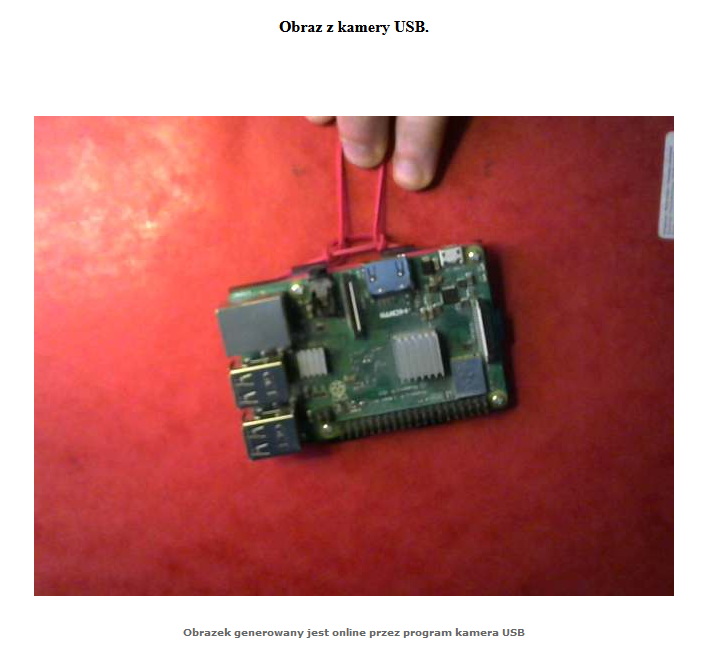
\includegraphics{aplikacja_testowa.png}
	   }
	\end{figure}
	\item Wylistuj urządzenia typu cap (kamery) i stwórz interfejs umożliwiający wybór po nazwie urządzenia (drivera) z którym chcesz sie połączyć
	\item Połącz się z wybranym urządzeniem i za pomocą odpowiednich komunikatów łączących się z driverami kamery - skonfiguruj ją.
	      \begin{itemize}
		      \item Za pomocą programu powinno dać się zmieniać opcje kamery (rozdzielczość obrazu, nasycenie, kontrast, ew. zoom, sterowanie kamera etc.)
		      \item Zapisz obraz z kamery w dowolnym formacie (wskazany JPG)
		      \item Zapisz obraz z kamery w postaci filmu AVI
	      \end{itemize}
	\item Rozbuduj program o:
	      \begin{itemize}
		      \item zmień tak program z zadania 3 aby generował stronę html z odświeżanym automatycznie obrazem z kamery
		      \item dodaj opcje która w przypadku gdy kamera potrzebuje swoich własnych sterowników automatycznie po włączeniu programu instaluje je; po poznaniu sterowników kamery należy znaleźć plik inf, które zostanie odpowiednio uruchomiony przez program (ShellExecute)
		      \item stwórz prosty detektor ruchu - poprzez analizę obrazu z kamery w czasie rzeczywistym (wystarczy sprawdzać zmiany koloru kilku punktów (pikseli), ćwiczenie można rozwinąć o najprostsze algorytmy wykrywające krawędzie etc.)
	      \end{itemize}
	\item Alternatywne metody wykonania zadanie (po uzgodnieniu z prowadzącym):
	      \begin{itemize}
		      \item AVICAP 32
		      \item wykorzystać Direct X (Direct Show)
		      \item wykorzystując WIA 1.0
		      \item wykorzystując WIA 2.0
		      \item wykorzystując WPD Automation Object Model
	      \end{itemize}
\end{enumerate}
\section{Wnioski}
\end{document}